% -*- mode: latex; mode: auto-fill; coding: utf-8; -*-

\chapter{Sky}
The sky is an essential part of an outdoor environment, whether it is
night, day, cloudy or clear sky plays an important role in setting the
mood of the scene. 
%Each of these different looking skies are composed
%of different phenomena that needs to be modeled and simulated by
%differently.
The sky is an ever changing part of an outdoor scene
and depends on many parameters including both the time of the day and
on the weather conditions.
%
This makes it a hard effect to simulate and visualize, but because it
is such a central part of an outdoor setting, it must be included in
the rendering.
%
One possibility is to simulate all important real world components
influencing the appearance of the sky. This could involve complex
weather forecast models or other large simulations, but because
there are so many complex phenomena influencing the skies appearance the
calculations of such models cannot be computed in real-time. Instead
we have chosen some of the skies most obvious visual effects and tried
to create believable visualizations of those.

When rendering a scene it is important that the overall LOD
matches to convince the user of our illusion. This means that if we
have a scene with high detailed objects, we also need to render the
sky in high detail. If we had a simple scene, then it could be enough to
simulate the sky by a simple light blue background color. This
approach works fine when used together with for example cartoon
shading. But as objects in the scene becomes more detailed and
realistic looking this simple approach makes the sky stand out. 
%
Simulating a more realistic looking sky can and have been done many
different way. Some authors use what is known as a \emph{sky box}
\citebook{page~338-339}{RTR2},
which is a technique that maps images of the sky onto a axis aligned
box. This box is so large that it contains the entire scene and by
moving the center of the box according to the camera position creates
the illusion of fare stretching planes by using simple images.
%
One problem with using a box when doing this, is that the edges
between the images on different faces of the box are apparent as
artifacts when looking directly at them. To get around this problem,
developers instead use a sphere or dome as the basic geometry, and
hence what is know as a \emph{sky dome}, when rendering the sky. The
main difference between these two approaches is texture mapping
the images. When mapping images onto a box a straight forward approach
can be used, but when using a dome this step becomes much more tricky.
%
Although the sky dome technique gives fine results, the sky remains
frozen in time, which makes it unrealistic when looking at it over
longer periods in time. 
%
So we have also take up the challenge of simulating or animating the
images which is to be mapped onto the sky dome.

\section{Sun}
Before we describe the sky dome we will introduce the source that lights
and hereby influences the entire scene. The only light source in our
scene is the sun, which is a directional light source that we move
around according to the time of day.

*** Lighting properties: shader on the dome, in the water, on the landscape...

\section{Sky domes}
We have chosen to using two sky spheres, one inner sphere for
rendering clouds as a black and white image with alpha transparency,
and an outer sphere to render a background color which can change
based on the time of day. We also include texture coordinate animation
of the cloud texture based on a simple wind model, so the clouds
change over time.

\subsection{Geometry}
We have tried two different ways on generating the sphere
geometry. The first method used was the traditional longitudinal/latitude
sphere commonly used for geographical maps. This
however gave very obvious image stretching artifact at the poles
because of oversampling in these regions. Instead we now use geodesic
spheres which consist of equilateral triangles. This sphere is
beautifully constructed by recursively subdividing the triangles of an
icosahedron until the required LOD is attained.

\subsection{Atmospheric dome}
What phenomena drives the coloring of the sky, making it so beautiful
with it shades of blue and red?
This is the questing asked by researchers studying 
\emph{atmospheric scattering}. Atmospheric scattering has been studied
in great detail and many complex theories and models has been
developed within the field. We however have chosen a simple technique
to model this complex process. This technique is based on a
\emph{color gradient} as described in \citeabook{abad2006}.

\begin{figure}[!h]
  \centering
  \subfloat[Color gradient.]{
  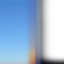
\includegraphics[width=5cm]{EarthClearSky2}
  \label{fig:sky-gradient}

  }
  \hspace{8mm}
  \subfloat[Star texture.]{
  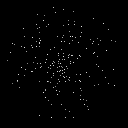
\includegraphics[width=5cm]{stars}
  \label{fig:sky-stars}
  }
  \caption{Textures used to color the atmospheric dome.}
  \label{fig:atmosphere}
\end{figure}

We use the color gradient in figure
\ref{fig:sky-gradient}, borrowed from the open source framework: 
Caelum\footnote{\url{http://www.ogre3d.org/tikiwiki/Caelum}}, to
color the fragments of the atmospheric dome. We use the
fragments height in the dome for texture mapping vertically on
the color gradient and the time of day in the horizontal
direction. This divides time into four periods: day, sunset, night,
and sunrise by first going from left to right, and then the
other way.
%
The white color seen on the right in figure \ref{fig:sky-gradient}
is alpha transparency, which is used at night to enable rendering of
stars. We render stars simple by pre-generating a black square image
with randomly placed pixels, painted shades of white, in a circle
round the center of the image as illustrated in figure
\ref{fig:sky-stars}. This images is then alpha blended with the color
gradient based on the three dimensional texture coordinates of the
atmospheric dome. The x and z coordinates are used (the y axis is up).

\subsection{Cloud Dome}
The cloud dome is simply used to map a cloud texture.

\subsubsection{Cloud texture}
We have chosen to use a procedural generated image to texture the
cloud dome. By take this approach we can generate very different
looking clouds by only altering a few parameters that is supplied to
the generation algorithm.
%
We have furthermore chosen a three dimensional image because this
eases texture mapping when the image is to be mapped onto the sphere.
%
To generate the cloud image we have been inspired by an Internet
homepage\footnote{\url{http://freespace.virgin.net/hugo.elias/models/m_clouds.htm}
  \\Be warned though, this homepage does not use Perlin noise as they
  say but value lattice noise.}
The page describe how to use procedural generation and
image layering/composition in combination to produce texture that
looks like real clouds.
Because procedural data generation is a large subject we have
dedicated a separate chapter for it, chapter \ref{chap:noise}. Here it
is enough to say that we generate a three dimensional texture which
can be tiled in all three dimensions.

\subsubsection{Texture mapping - animation}
The basic texture mapping scheme, is to put the three dimensional
texture into a unit cube, and use texture coordinates based on the
unit sphere to make a direct mapping which avoids texture stretching.
%
If we only did this, the a large portion of the generated texture
would not be used.
%
So besides the basic texture mapping scheme, we have introduced
texture coordinate animation. This has been done by modeling the wind.

\subsubsection{Wind simulation}
We have implemented a simple wind simulation algorithm which is
inspired by Brownian motions. \citebook{}{}
The algorithm works by having a two wind directions referred to as the
current and future direction. The future direction is generated
randomly based on the current direction and is normal distributed
around this. The wind is then changing progressively by interpolating
linear between these based on time. When the future wind direction is
reaches we overwrite the current by the future direction and generate
a new future wind direction.

%%% Local Variables:
%%% mode: latex
%%% TeX-master: t
%%% TeX-PDF-mode: t
%%% End:

